\documentclass[10pt]{article}
\usepackage[utf8]{inputenc}
\usepackage{graphicx}
\usepackage[margin=1in]{geometry}
\linespread{0.9}
\title{Climate Trend Analysis: Is Florida Getting Warmer?}
\author{Bowen Duan}

\begin{document}

\maketitle

\section{Introduction}
This report examines historical temperature data to answer the question: is Florida warming? By analyzing the temperature trends in Key West, Florida, I conclude that there is an upward trend in temperatures over the 20th century.

\section{Methods}
I conducted a permutation analysis to calculate the correlation coefficient between time and temperature, accounting for the serial dependence in the time-series data. This method shuffles the temperature data points and recalculates the correlation coefficient 1000 times to create a distribution of correlation coefficients under the null hypothesis of no relationship between time and temperature.

\section{Visualization}
\begin{figure}[ht]
\centering
\begin{minipage}{0.4\textwidth}
  \centering
  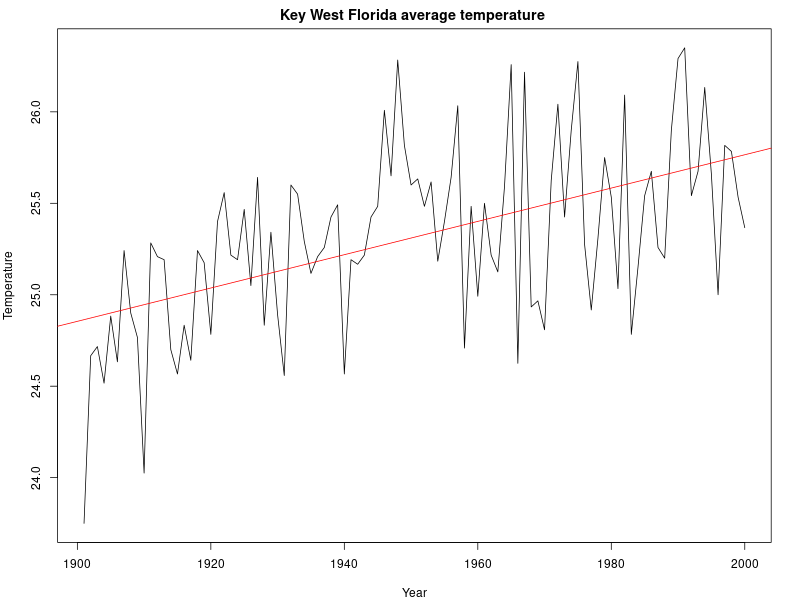
\includegraphics[width=\linewidth]{../data/results.png}
  \caption{This can be learned by looking at the trend line added to the graph. The trend in average annual temperatures for Key West shows a significant increase in average annual temperatures since the 20th century, showing that Key West's climate is warming.}
  \label{fig:temp_trend}
\end{minipage}
\hfill
\begin{minipage}{0.4\textwidth}
  \centering
  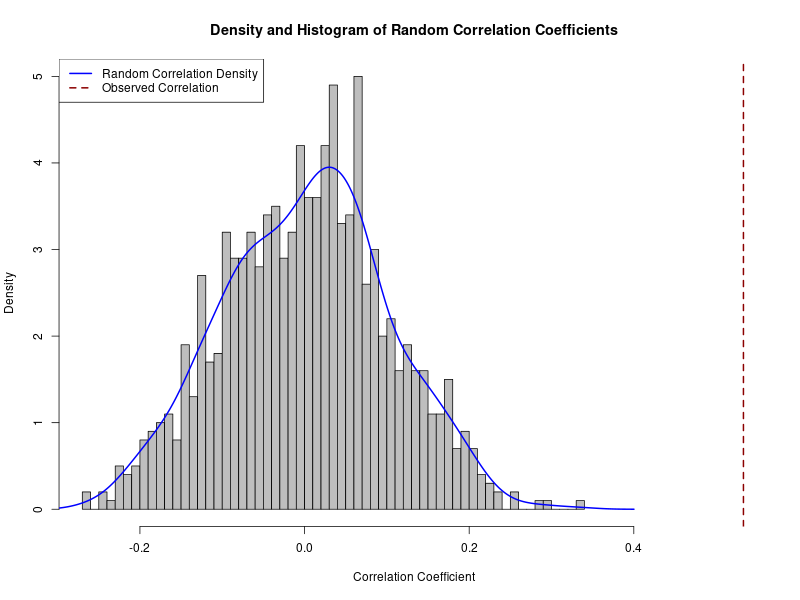
\includegraphics[width=\linewidth]{../data/cor.png}
  \caption{It is clear from the histogram that the random correlation coefficient is much smaller than the observed correlation coefficient, so it can be concluded that the value of p value is very small}
  \label{fig:corr_dist}
\end{minipage}
\end{figure}

\section{Conclusion}
The statistical analysis clearly indicates that Florida is experiencing a warming trend. The observed correlation coefficient significantly exceeds the distribution of coefficients under the null hypothesis, with a p-value less than 0.0001. This analysis confirms that the temperatures in Key West have risen significantly over the past century.

\end{document}

